\documentclass[12pt]{report}
\usepackage{url}
\usepackage{graphicx}

\author{Ken Hoff \\ University of Colorado at Boulder \\ \texttt{kendall.hoff@colorado.edu} 
\\ \\ Advisor \\	\\ Alexander Repenning, Professor, University of Colorado 
\\ \\ Committee \\	\\ Alexander Repenning, Professor, University of Colorado
					\\ Michael Eisenberg, Professor, University of Colorado
					\\ John Bennett, Professor, University of Colorado
					\\ Julien Lynge, Research Faculty, NOAA}
\date{\today}
\title{Improving Educational Game Design Methods: A Rubric to Assess the Engagement and Educational Value of Educational Games
}

\begin{document}

\maketitle

\begin{abstract}

Existing educational games lack the combination of education and engagement. The objective is to research, synthesize, and test a more effective educational design method. The procedure is to research current literature and existing effective educational games, synthesize an educational game design rubric based off of this research, then apply this method to known educational games. Amazon's Mechanical Turk will be used to gather large amounts of data about the consistency of this rubric, after which the data will be collated and analyzed.

\end{abstract}

\tableofcontents

\section{Problem}
	Educational games lack the combination of education and engagement. The standard is “cheesy” games, where the content being taught is either uninteresting or unrelated to the type of play. A good example is Math Blaster; players answer simple arithmetic questions to fill up their energy, which they then use to shoot space debris. These “games” are usually just homework problems, either included as an unrelated component inside the game, or interspersed between gameplay segments in a quiz format.

\section{Thesis Statement/Solution}
	I'm going to synthesize an education game design method by creating a list of attributes that educational games should have a high degree of in order to be effective and engaging. The list is not a set of standards, but a set of guidelines; it is possible (though unlikely) for a game to contain all of the attributes and still be ineffective, or for a game to have none of the attributes and be very effective. It is simply meant to infer that game designs that contain these elements are more likely to be effective and engaging educational games.

\section{Approach} 
	I'll begin by examining current educational game design methods, through research of published literature. I'll then synthesize my own educational game design method, a list of attributes found in effective and engaging educational games, influenced heavily by my research and findings. Afterwards, I'll attempt to apply my method to existing educational and semi-educational games, and see if the most effective educational games correlate to my design method. In contrast, ineffective educational games won't correlate at all to my design method.

\section{Research}
	\subsection{Edutainment vs Educational Games}
		\subsubsection{Bloom's Taxonomy}

			Bloom's Taxonomy is one of the most widely cited classifications of learning. It provides milestones for three different domains of learning: Psychomotor, Affective, and Cognitive.

			The first domain, Psychomotor, deals with the ability to perform intricate physical tasks, like hammering a nail or operating a complex machine or instrument. Games are currently very good at teaching concepts within the Psychomotor domain. The best examples are ones where the game provides a near-simulation to the task being performed in real life. Music games like Guitar Hero and Rock Band improve coordination and motor control while playing an instrument. Simulation driving games like Forza and Gran Turismo provide players with continuous feedback to help them learn the correct response to stimulus given the car they are driving, to help them improve their driving skills. Other examples include any game that improves motor control; Kinect's Dance Central improves player's bodily movements, and even first person shooter games like Halo or Call Of Duty improve player's hand-eye coordination.

			The Affective domain is one that is far harder for games to address. It deals with learning empathy, emotion, and includes things that are commonly learned through interaction with people and not necessarily through formal education. Games commonly expose players to this in two ways. The first is through game narrative, where players are exposed to characters, situations, and choices where they observe and learn about the human condition. Games with extreme character development (Mass Effect, The Walking Dead) typically explore human choices in great detail. There are also extremely minimalistic games that communicate powerful empathic ideas without a large amount of gameplay or graphics, or conversation (Thomas was alone, Journey), as well as completely narrative-based, choose-your-own-adventure Twine games that address extremely empathic concepts (Howling dogs). The second is through putting players in situations with other players where they will need empathy and skills from the Affective domain in order to solve their problems. All multiplayer games facilitate this to some degree, but puzzle games (Portal, LittleBigPlanet), and MMO's (WoW, EVE Online) generally encourage players to communicate, negotiate, and work together to achieve a common goal.

			When we think of educational games, we commonly think of the Cognitive domain. The Cognitive domain deals with knowledge of facts, associations, and mechanics, and typically consists of the material that educators attempt to teach in schools. This is also the domain that games attempt to address the most; being able to communicate these concepts effectively would reduce the amount of material educators would need to teach, allowing them to focus on more complex concepts. Because games in the Psychomotor domain are well traversed, and games in the Affective domain are far more nebulous as to measuring their educational value, we will be focusing exclusively on the Cognitive domain.



			\textbf{image}

			\subsubsection{Educational Games, Not Edutainment}
				It's also important for us to differentiate between edutainment and educational games. For this paper, we're going to define edutainment as the simple gamification of a task. The purpose of edutainment is to increase the player's skill at something by getting them to play a game; the player mimics or actually does the skills within the game, and the game rewards them and keeps them engaged in order to continue increasing their skill. These kinds of games, while effective, are ineffective at teaching complex concepts and systems. For that purpose, we use educational games; they have the more rewarding task of teaching complicated content, but it is far more difficult to do so, as they can't utilize the “skill and drill” method of education. We're going to focus primarily on educational games in this paper.

	\subsection{Tangential Learning}

		In their paper on “Serious Games and Learning,” Breuer and Bente (2010) outline a method called “Tangential Learning.” Originally presented as part of the “Extra Credits” video series online (Floyd and Portnow, 2008), the presenter gives us a method for which we can encourage significant learning using games. The theory is that, given the proper incentive, players will engage in a form of self-education separate from the game environment.
		
		They base this on the principle that we're able to recall and understand material that we're more interested or passionate about, rather than material that is uninteresting or boring to us. The same principle applies to video games; if we are interested in the context of an educational game, we're far more likely to remember that instead of the content being taught as part of it. The example Extra Credits uses is geography; it's easy for some players to draw the entire map of Azeroth from memory, but they're unable to properly identify US states.
		
		The most prominent field that this could be applied to is history; as most games are set in the past, such as Ancient Rome or World War II, it would be easy for players to learn more about history on their own simply because they were playing the game in the appropriate context. There are other contexts that players can be placed in, in order to educate about other topics. Players in music games can self-educate on music theory and different musical genres, and players in space simulations might self-educate on spaceflight and astronomy. 
		
		However, there are numerous other ways players can be educated apart from being placed in the context of the educational goal. An easy-to-implement way would be to include facts as part of the loading screens in the game; instead of having game tips or strategies, designers could include interesting bits of external information to help players retain information. Also, designers can include subtle references to real-life objects within their games. Extra Credits gives the example of Sephiroth from Final Fantasy, or the Excalibur and the Masamune. By naming characters or objects after real-life characters or objects, designers can encourage players to go out and seek the origin of the character or object; it also helps to have once object in a group be something that's easily recognizable, so that players immediately know that other objects in the group are referential to the real world.
		
		Another excellent way to integrate tangential learning into games is by including an in-game encyclopedia, where players don't even have to leave the game to explore more about the topic they're interested in. Usually, these encyclopedias include information related to playing the game; the stats of an object, or the rules of the game. However, some include information that isn't related to playing the game, like the history or origin of an object or character. A notable example of this is the game Civilization, which includes the Civilopedia, a reference to every unit, building, and wonder in the game, as well as other information related to it. An easy way for games to integrate this would be just including Wikipedia links to every object in the game that has real world roots.
	
	\subsection{Flow}

		Dondlinger (2007) explains why it's extremely important to give players the perception of free will. In educational games, we don't want to give the players no direction as to where to go within the game; we risk players missing the educational goals, and worse, becoming frustrated with the lack of progress. Conversely, we don't want to overly guide the players; too much hand-holding results in the game stifling creativity, as well as not allowing players to really “learn by doing.” It's important for us to give them the illusion of having an open world, where almost any actions are possible, in order to allow players to experiment and learn by doing.

		In parallel to the illusion of free will is the concept of ‘flow.' In games, we want to the player to experience just the right difficulty; games that are too hard will be frustrating, and games that are too easy will be boring. The same is true of education and educational games; material that is far beyond the comprehension of the learner won't be retained, but material that the learner has already covered sufficiently will be boring. We need to maintain a level of difficulty to our game that Csikszentmihalyi (1997) calls ‘flow.' When players are in a state of ‘flow,' the game provides to them a clear set of inputs and outputs; material that they are somewhat familiar with, but also obscure enough to encourage to players to try several options in order to solve the problem.

		Following the concept of ‘flow,' we can extrapolate the concept of ‘adaptive difficulty.' It's logical to assume that games that continually adapt their difficulty level to the players will be more effective in retaining the player's interest and educating the player than games that have a fixed difficulty curve. However, not every game can implement adaptive difficulty effectively; games need the players to continuously attempt problems and give feedback on how well they're doing to ascertain how well the difficulty matches up to the player.

	\subsection{Play}

		Similar to the illusion that players have a seemingly limitless game world to interact with is the concept of ‘play.' Paras (2005) defines a world where play can happen simply as a world with a series of constraining rules. We don't want the rules to be too constraining, because then we inhibit creativity and discourage alternative solutions to problems, but at the same time, we want the rules to be constraining enough to guide the player towards the solution and mimic the rules of the real world.
		
		The way the game guides players around these rules is extremely important. If the game gives the player copious amounts of tutorials and guidance as to what they can or can't do in the game, the player won't learn them as well. This isn't to say that the player should be encouraged to break the game rules, but instead to encourage the player to explore the world's rules; they won't understand what will and won't work unless they encounter it on their own and are enabled to learn from it.
	
		The game also shouldn't penalize the player for exploring the boundaries of the game world, as it would discourage them from trying new things and discovering additional boundaries. However, we still need to encourage players to solve problems within the game world without breaking any boundaries, just to ensure that they understand the world that they're playing in; that's why rewarding the players for not breaking any rules works much better than penalizing the player for breaking rules.

\section{Findings}
	\subsection{Design Rubric}
		What follows is a list of properties that make up the educational game design, created by researching and synthesizing properties of existing educational games. Games are not required to have all or any of these properties, but the hope is that games with more of these properties will be considered more effective and engaging educational games. Certain sections of the rubric are left blank, but properties of the section can be extrapolated from adjacent sections.
	\subsection{Rubric Overview}
	\subsection{Rubric Details}
		(graphics go here)

		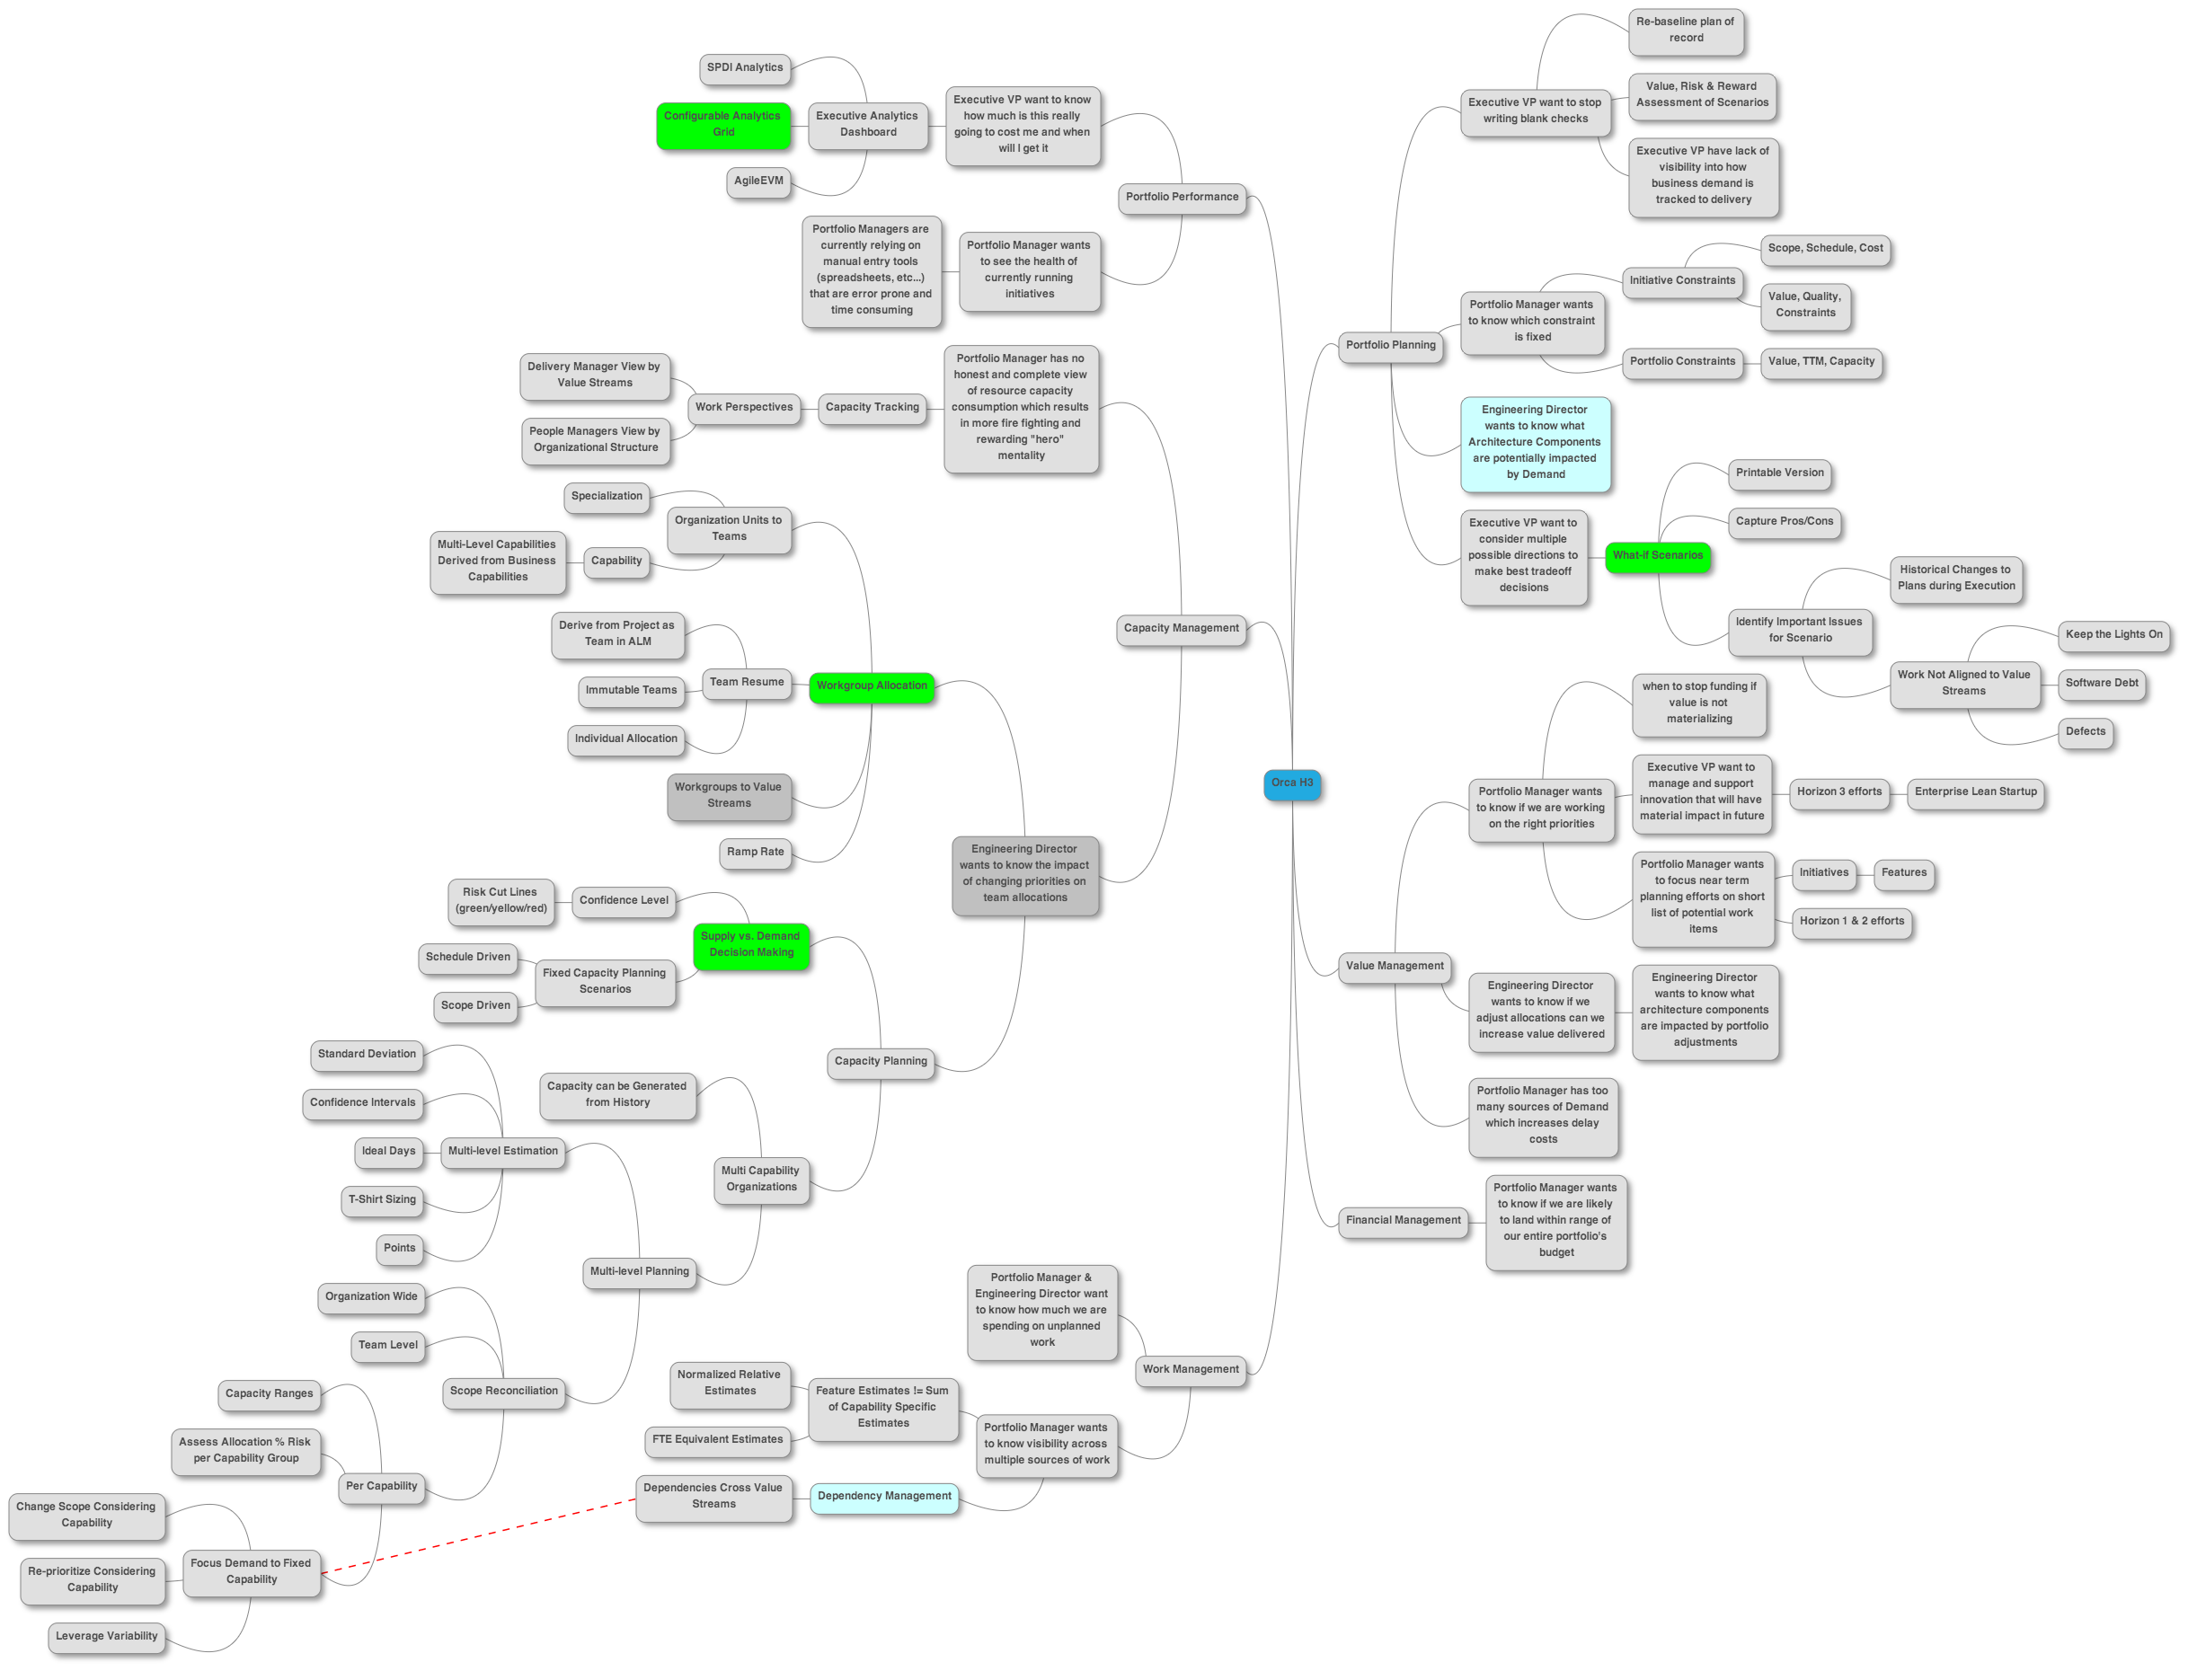
\includegraphics[width = \textwidth]{./Orca_H3.png}

		

	\subsection{Games Overview}
		chart
	\subsection{Games Details}
		\input GameSummaries

\section{Conclusion}
	This rubric is moderately effective. It places heavy emphasis on self-paced, self-motivated learning, which is most easily demonstrated by the high scores received by games that encourage a high amount of tangential learning. However, this means that games that are not explicitly educational rank highly, like Civilization and Kerbal Space Program. However, the emphasis on adaptive difficulty and feedback means that many traditional games, like Carmen Sandiego and Math Blaster, rank lowly on the scale. In addition, games that focus on exploration and play rank highly, like the original Robot Odyssey and SimCity 3000.
\end{document}